\documentclass[12pt,serif,draftclsnofoot,onecolumn]{IEEEtran}
\usepackage{color}
\usepackage{setspace}
\usepackage{url}
\usepackage{graphicx}
\usepackage{listings}
\singlespacing

\lstdefinestyle{customc}{
	belowcaptionskip=1\baselineskip,
	breaklines=true,
	frame=L,
	xleftmargin=\parindent,
	language=C++,
	showstringspaces=false,
	basicstyle=\footnotesize\ttfamily,
	commentstyle=\bfseries\color{black},
	identifierstyle=\color{blue},
	stringstyle=\color{orange},
}
\lstset{escapechar=@,style=customc}
\newcommand{\HRule}[1]{\rule{\linewidth}{#1}}
\begin{document}
	\begin{titlepage}


	\title{ \normalsize \textsc{}
			\\ [2.0cm]
			\HRule{0.5pt} \\
			\LARGE \textbf{\uppercase{Final Report}}
			\\ \normalsize \textsc{Accurate Earth Orbit}
			\HRule{2pt} \\ [0.5cm]
			\normalsize \today \vspace*{5\baselineskip}}
	\date{10/16/2016}
	
	\author{Steven Silvers \\
			silverss@oregonstate.edu \\
			Oregon State University \\
			CS 450 Intro to Computer Graphics}
	\pagenumbering{gobble}	
	\maketitle
	\end{titlepage}
	\tableofcontents
	\newpage
	\pagenumbering{arabic}
	\section{T-Shirt}
	\par
			I would like my project to be considered for one of the Vulkan T-shirts. My size preference is large, followed by medium followed by extra-large.
	\newline
	\section{Proposal}
	\par
			While similar to the popular solar system project, this project will only involve the Earth's orbit around the sun and the moon's orbit around the earth. The Earth and moon orbits will both be to scale and follow their accurate elliptical paths, which will be a difficult transformation challenge. Getting an accurate speed of the orbit is difficult enough with a circular orbit, so going on an elliptical path provides an even greater challenge. The planets will also be transformed to rotate on their axes as they would in real life.
	\newline
	\par
			Textures will be applied to the Sun, Earth and moon to give the model a realistic look. The only source of light will be the sun to make this model as accurate as possible. I plan to be able to show eclipses with this model to add difficulty to the lighting aspect of the project.
	\newline
	\section{What was done}
	\par	
			For my final project I created a Sun-Earth-Moon model, as detailed in my project proposal while also following the added guidelines on the course website. These guidelines included exaggerating the distances and some of the sizes of the objects in the system so that it would fit nicely in a single viewing window, as if it were to be used as an educational tool.The other guidelines were to use good textures for the Sun Earth and Moon, as well as adding a viewing option from Earth looking out at space, and a viewing option from the Moon looking out at space.
	\newline
	\par
			My plan was to get the scene for the outside viewing window rendered and displaying the way I wanted it to before attempting to tackle the other two viewpoints. I did this by first drawing a sphere at the origin as my sun. When the Sun was finished I then added the Earth and the Moon as well. Once these were drawn and textured I began working on how I wanted the animation cycle to work.
	\newline
	\subsection{Outside View}
	\par		
			 I decided that the best approach would be to use the animate code that we had been given in previous projects, and make one full animation cycle to be an Earth year. Setting a full cycle to an Earth year made calculating the other rotations and transformations quite simple. I learned exactly how often the Moon completes an orbit of the Earth, how long it takes to rotate on its axis, and how long the Sun takes to rotate on its axis. These amounts were typically measured in Earth days, for example it takes the Sun approximately 35 days to complete a full rotation at its axis, so the calculation 365/35 gave me the time coefficient of 10.4 to use for the glrotatef() function.
	\newline
	\par
			After these calculations were made, I had a Sun-Earth-Moon model that had the earth following a circular orbit around the Sun, the Moon orbiting the Earth and no special lighting created.The next step to finishing this viewpoint was to put the Earth on an elliptical orbit about the sun. This was done using the following code for the Earth's transformations:
	\newline
	\lstinputlisting[language=C++, firstline=882, lastline=890]{sample.cpp}
			As you can see the X axis and Z axis translations are altered using sin/cos based on the Time variable. These translations create the elliptical path that is visible in Figure 1.
	\begin{figure}[h]
		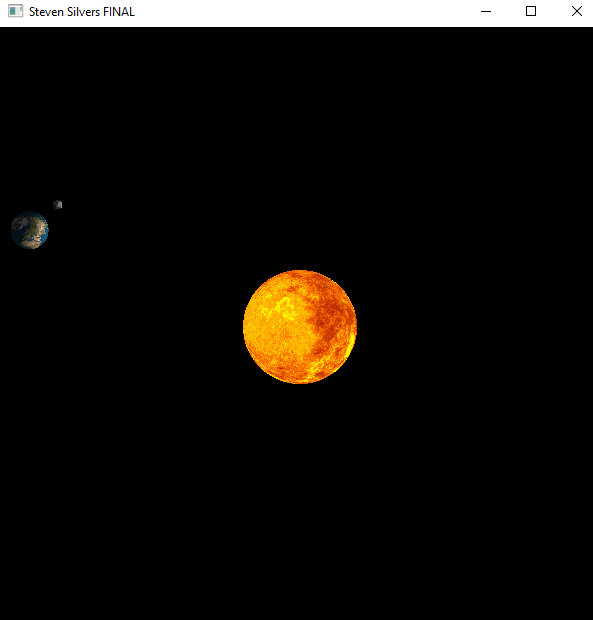
\includegraphics[scale=.5]{cap3}
		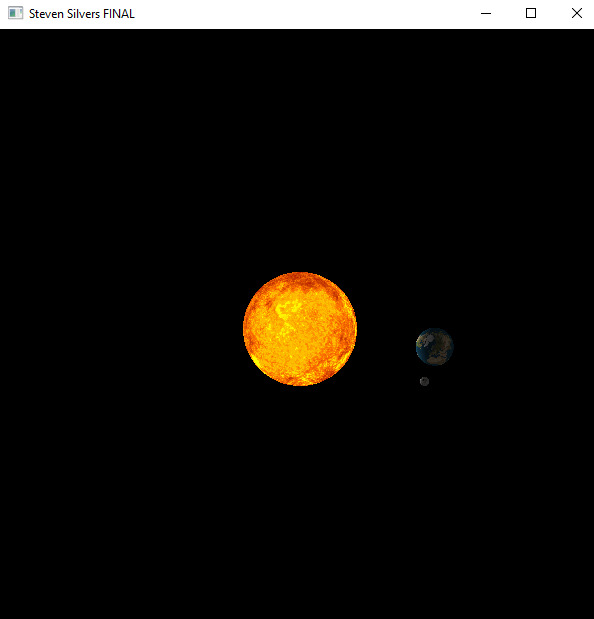
\includegraphics[scale=.5]{cap1}
		\caption{elliptical path of the Earth}
	\end{figure}
	\newline
			I elected not to put the moon on an elliptical path due to the exaggeration of distances in my simulation. Using a circular path for the Moon makes the interaction between the Moon and Earth easier to do and look less cluttered in the end. However, the size of the moon is 1/4 that of the Earth, which is reflected accurately in my system
	\newline
	\par
			The final step was to enable lighting and make the Sun a point light shining on the Earth and Moon. I achieved this by using the functions given in the lighting project earlier this term to create the light, with slight modification to add ambient light so that the dark sides of the Earth and Moon were still visible. I initially had trouble with the lighting because I forgot to modulate the textures, so no matter what I tried with altering my point light the change in lighting was still not reflected in the textured objects of the system.
	\newline
	\subsection{Oregon View}
	\par
			Creating this viewpoint caused a lot of trouble and a few long nights. When I first approached the problem, my idea was to just draw the objects like they were for the outside view and then transform the eye location and look at values with those objects. This proved to be futile as figuring out that kind of matrix transformation would ultimately be too complicated. 
	\newline
	\par
			I stopped to think about what viewing from Oregon would look like, and realized that when I stand outside looking up, from my perspective I'm not the one that is moving, the Sun and the Moon are the ones that are moving around me. This gave me the idea that for the Oregon viewpoint I should make the camera and the Earth stationary, and rotate the Moon and the Sun around the Earth. 
 	
	\begin{figure}[h]
		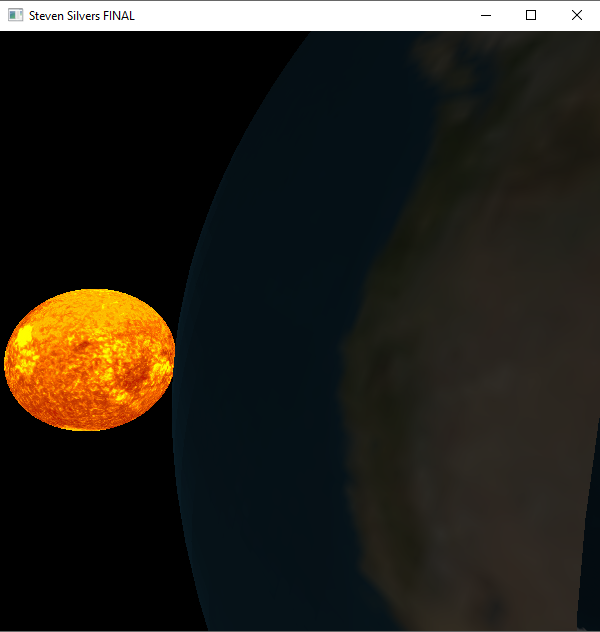
\includegraphics[scale=.67]{cap2}
		\caption{Watching the Sun set from Oregon viewpoint}
	\end{figure}

	\par
			I decided it would be easiest to put the Earth at the origin and rotate it so that the normal vector from Oregon's location on Earth would be about the same as the positive Z axis. This led to some quick guess and check work to find the best location for the camera's eye near the Earth, as well as the creation of some temporary test objects so I wasn't starring at just blackness. Since just staring out from Oregon waiting for the Sun and Moon to pass by, I included functionality to rotate the camera's eye so that we could also look side to side, as demonstrated in figure 2.
	\newline
	\subsection{Moon View}
	\par
			The Moon viewpoint went quite smoothly once the Earth viewpoint was figured out and completed. During my research I came across the fact that the Moon has a synchronous orbit about the Earth. The effect of this is that the same side of the moon always faces the Earth, meaning the Sun would be the only moving object in my system besides the Earth rotating.
			
	\begin{figure}[h]
	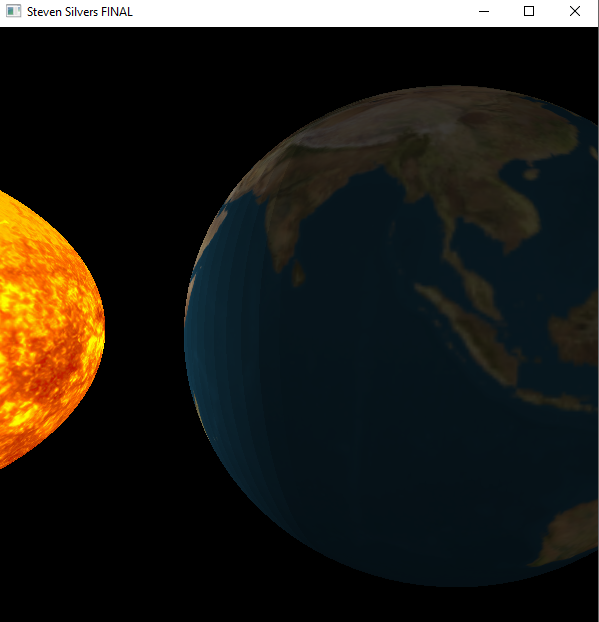
\includegraphics[scale=.67]{cap4}
	\caption{Looking at the Earth from the Moon}
	\end{figure}

	\par
			Exaggeration was again used in the distances from the Moon to the Sun and Earth, but they were kept consistent with the other viewpoints. The same camera functionality from the Earth viewpoint was included so that the user can look around while on viewing from the Moon.		
	\newline
	\section{Changes from Proposal}
	\par
			All changes in my project are either added functionality or to comply with the additional notes on the course website. As mentioned previously the distances between the three bodies is not to scale, nor is the size of the sun to the Earth and Moon. I elected to not do shadowing like I stated I wanted to in my proposal, as the notes on the course site made this sound more difficult than I would be capable of doing. I added quite a bit of functionality to make my project more user interactive and easy to work with.
	\newline
	\par
			Since it was getting boring waiting for my simulation to complete an orbit to make sure it was functioning properly, I added the ability to speed up and slow down the simulation by pressing 'I' or 'D' on the keyboard. The different viewpoints are also toggled using the keyboard, 'M' for Moon and 'E' for Earth, and 'R' to call the reset function which defaults to the outside viewpoint. A freeze ability was also added, this was just the same freeze functionality from previous projects. Camera control was added to get a better look at the systems, all three viewpoints can rotate the scene and the outside viewpoint can also zoom in and out.			
	\newline
	\section{What I learned}
	\par
			I think the biggest thing I learned from this project isn't even necessarily directly related to computer graphics. Making the realization that changing your perception within or about a system can completely open up new possibilities is something I learned when trying to make the additional viewpoints. I'm sure if I kept working and made endless mathematical calculations I could've had a moving camera eye, but instead it ended up being a quite simple solution with equal or even better results. While I did know that space was mostly just one space, researching the actual distances woke me up to just how far away everything is and why making those to scale in this project would make it less fun to play with.
	\newline
	\par
			I leatned a lot more about our solar system than I initially thought I would. Things like how quickly the Sun rotates varies from place to place on the Sun, or that in our solar system almost everything orbits the Sun in the anticlockwise direction. It was information like this that helped me make sure that certain details were correct, like the Sun rising in the East when using the Oregon viewpoint.
\end{document}